\textbf{Beispiel 2}\\ \\
a)\\ \\
Die Anzahl der Freiheitsgrade, die dieses System komplett beschreiben lautet 1, weil es hier nur eine Größe existiert die sich durch eine Bewegung des Systems ändert.\\ \\
b)\\ \\
Freigeschnittene Brücke:
\begin{figure}[h]
	\centering
	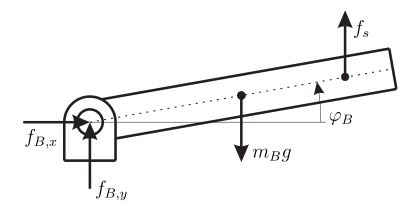
\includegraphics[width= 12.5cm]{tikz/19_05_2017_2b}
\end{figure}
\newline
Das gesuchte Kräftegleichgewicht lautet
\begin{align*}
	\textbf{e}_x &: f_{B,x} = 0 \\
	\textbf{e}_y &: f_{B,y} - m_Bg + f_s = 0
\end{align*}
und das Momentengleichwicht lautet
\[
	\textbf{e}_z : -m_Bgl_B\cos(\varphi_B) + f_sl_s\cos(\varphi_B) = 0
\]
Um die Seilkraft zu bestimmen muss nur das Momentengleichwicht in Betracht gezogen werden.
\begin{align*}
	-m_Bgl_B\cos(\varphi_B) &+ f_sl_s\cos(\varphi_B) = 0 \\ 
	 f_sl_s\cos(\varphi_B) &= m_Bgl_B\cos(\varphi_B) \\
	 f_s &=  m_Bg\frac{l_B}{l_s}
\end{align*}
\newpage
\noindent
c) \\ \\
Freigeschnittener Träger:
\begin{figure}[h]
	\centering
	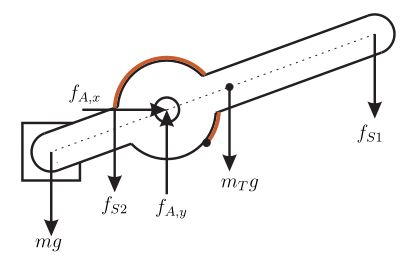
\includegraphics[width= 10 cm]{tikz/19_05_2017_2c}
\end{figure}
\newline
Hier lautet das Kräftegleichgewicht
\begin{align*}
	\textbf{e}_x &: f_{A,x} = 0 \\
	\textbf{e}_y &: -mg - f_{S2} + f_{A,y} - m_Tg - f_{S1} = 0
\end{align*}
und das Momentengleichgewicht
\[
	\textbf{e}_z: mgl_m\cos(\varphi_B) + f_{S2}R - m_Tgl_T\cos(\varphi_B) - f_{S1}l_s\cos(\varphi_B) = 0
\]
Um wieder die fehlende Seilkraft zu bestimmen muss wieder nur das Momentengleichwicht betrachtet werden. Daher lautet diese
\begin{align*}
	mgl_m\cos(\varphi_B) + f_{S2}R - m_Tgl_T\cos(\varphi_B) - f_{S1}l_s\cos(\varphi_B) = 0 \\
	mgl_m\cos(\varphi_B) + f_{S2}R - m_Tgl_T\cos(\varphi_B) - m_Bgl_B\cos(\varphi_B) = 0 \\
	f_{S2} = \frac{m_Bgl_B + m_Tgl_T - mgl_m}{R}\cos(\varphi_B)
\end{align*}
d)\\ \\
Um die gesuchte Masse zu bestimmen, muss man beachten das die Kraft $f$ gleich der Kraft $f_{S2}$ sein, d.h. man muss die beiden gleichsetzen. Daraus folgt
\begin{align*}
	\frac{m_Bgl_B + m_Tgl_T - mgl_m}{R}\cos(\varphi_B) = 0 \\
	m_Bgl_B + m_Tgl_T - mgl_m = 0 \\
	m = \frac{m_Bl_B + m_Tl_T}{l_m}
\end{align*}
\newpage
\noindent
e)\\ \\
Die Formel zu Berechnung des Massenträgheitsmoment kann der Formelsammlung entnommen werden.
\begin{align*}
	\varTheta_B &= \int_{\mathcal{V}}r^2\text{d}m = \rho \int_{\mathcal{V}}r^2\text{d}V \\
	&= \rho b \int_{0}^{l}\int_{-\frac{d}{2}}^{\frac{d}{2}}(y^2 + z^2)\text{d}z\text{d}y \\
	&= \rho b \int_{0}^{l}\left(y^2z + \frac{z^3}{3}\right)\biggl|^{\frac{d}{2}}_{-\frac{d}{2}}\text{d}y \\
	&= \rho b \int_{0}^{l}\left(y^2\frac{d}{2} + \frac{d^3}{16} + y^2\frac{d}{2} + \frac{d^3}{24}\right)\text{d}y \\
	&= \rho b \int_{0}^{l}\left(y^2d + \frac{d^3}{12}\right)\text{d}y \\
	&= \rho b \left(\frac{y^3}{3}d + \frac{d^3}{12}y\right)\biggl|^{l}_0 \\
	&= \rho b \left(\frac{l^3}{3}d + \frac{d^3}{12}l\right)
\end{align*}
Mit $m_B = \rho lbd$ folgt
\[
	\varTheta_B = m_B\left(\frac{l^2}{3} + \frac{d^2}{12}\right)
\]
f)\\ \\
Wenn nun das Seil 1 reißt wird die Brücke fallen. Da sich hier dann um eine Drehbewegung handelt besitzt die kinetische Energie der Brücke nur einen rotatorischen Anteil und lautet somit
\[
	T = \frac{1}{2}\varTheta_B\dot{\varphi}^2_B
\]
Die potentielle Energie zum Zeitpunkt $t = 0$ lautet
\[
	V = m_B g l_B \sin(\varphi_0)
\]
Da die Energieerhaltung erfüllt sein muss folgt für die gesuchte Winkelgeschwindigkeit
\begin{align*}
	T &+ V = 0 \\
	\frac{1}{2}\varTheta_B\dot{\varphi}_B^2 &+ m_B g l_B \sin(\varphi_0) = 0 \\
	\dot{\varphi}_B &= - \sqrt{\frac{2m_Bgl_B}{\varTheta_B}\sin(\varphi_0)} 
\end{align*}